\documentclass[12pt,a4paper,oneside]{article}
\usepackage[latin1]{inputenc}
\usepackage{amssymb, amsmath, amsfonts, mathbbol}
\usepackage{graphics,graphicx,epsfig,ulem} 
\usepackage{multirow} % Allows multirow tables
\usepackage[margin=2.5cm]{geometry} % Set page margins
\usepackage{cite} % For better citations
\usepackage{url} % For better URLs

% Fonts
\usepackage[T1]{fontenc}
\usepackage{cmbright}

% Double spacing
\usepackage{setspace}

% Headings
\pagestyle{myheadings}
\markboth{}{Interim Report: Running Coupling in the Standard Model and Beyond}

\begin{document}

\title{Running Coupling in the Standard Model and Beyond\\Interim Report} 
\date{\today}
\author{Jonathan Arnold\thanks{Physics Department, University of Durham, South Road, Durham, DH1 3LE}}

\maketitle

%\begin{abstract}
%\end{abstract}

%Start double spacing
\doublespace

\section{Introduction}
One of the greatest triumphs of 20th Century physics has been the Standard Model (SM). In it, the principle of local gauge invariance has been used to show that electromagnetic, strong and weak interactions can be modelled using the SU(3)$\times$SU(2)$\times$U(1) gauge groups to spectacular accuracy\cite{sm-1,sm-2}. Despite these great successes, it has become evident that the Standard Model does not describe a number of phenomena accurately, such as the observations of neutrino oscillations \cite{neutrinos} and matter-antimatter asymmetry \cite{mass}; as such, it is reasonable to find a more encompassing theory that includes the Standard Model within it.

It has been widely noted \cite{amaldi, running-2} that the coupling strength for the electromagnetic, strong and weak interactions vary (``run'') depending on the energy scale, due to renormalisation. The running of these couplings allows us to suggest that they would take the same value (``unify'') at a certain energy scale. This unification would admit the possibility of a Grand Unified Theory (GUT), capable of describing all three interactions as a single unified interaction. A number of GUTs have been proposed \cite{pdg} and all require a unification point to exist, although how this unification is broken is theory-dependent.

This project aims to investigate the scales and conditions required to unify electromagnetism, strong and weak interactions into a single GUT. As well as this, a number of popular GUTs are analysed to find experimental predictions available to test in the current or next generation of colliders.

\subsection{Outline of the Project}
The first aim of the project is to replicate results for the SM and Minimal Supersymmetric Standard Model (MSSM) obtained by \textit{Amaldi et al.} \cite{amaldi}, updating this paper by using the 2002 world-averaged values from the \textit{Particle Data Group} \cite{pdg}, as well as provide further insight into the results obtained.

Once obtained, the aim is to analyse a number of Grand Unified Theories to determine whether unification is admitted in the theory (in accordance with experimental data) and if so the energy scale at which the unification is found.

\section{Theory}

\subsection{Analytical Theory}

Almost all theories of interaction in particle physics admit solutions where infinities become problematic for further calculation. In order to combat these anomalies, we can renormalise the theory: this uses symmetries of scale to define the theory at a different observation scale, based on its particular structure at a well-defined scale. Using a procedure outlined by \textit{Bogoliubov and Shirkov} \cite{bogoliubov}, we can arrive at a \textit{beta function} for the theory, which allows us to determine the strength of an interaction $g$ at a certain scale $\mu$:
\[
\beta (\mu) = \mu \frac{\partial g}{\partial \mu} \:.
\]

A running coupling arises when one renormalises the Standard Model or MSSM \cite{renorm, renorm-2}: in each of its sectors, the coupling strength varies with energy scale. Considering one- and two-loop diagrams, the RG equations are \cite{amaldi}
\[
\mu \dfrac{d}{d \mu} \alpha_i (\mu) = \dfrac{1}{2 \pi} \left( b_i + \sum_{j=1}^{3} \dfrac{b_{i j}}{4 \pi} \alpha_j (\mu) \right) \alpha_i^2 (\mu)
\]
where $\alpha_i (\mu)$ gives the coupling strength at an energy scale $\mu$, and $i = 1,2,3$ denotes the U(1), SU(2) and SU(3) sectors of the Standard Model respectively. The constants $b_i$ and $b_{ij}$ are model-dependent constants for one-loop and two-loop corrections respectively. This can be rewritten as
\begin{equation}
\mu \dfrac{d}{d (\ln \mu)} \alpha_i^{-1} (\mu) = -\dfrac{1}{2 \pi} \left( b_i + \sum_{j=1}^{3} \dfrac{b_{i j}}{4 \pi} \alpha_j (\mu) + \mathcal{O}(\alpha_j^2) \right) \:,
\label{eqn:rg}
\end{equation}
where we adopt ``big O'' notation to denote higher order terms.

We repeat the procedure outlined by \textit{Amaldi et al.} \cite{amaldi}: we define the couplings as
\[
\alpha_1^{-1} = \dfrac{3}{5} \dfrac{\cos^2 \theta_W}{a} \:, \quad
\alpha_2^{-1} = \dfrac{\sin^2 \theta_W}{a} \:, \quad
\alpha_3^{-1} = \dfrac{1}{a_s}
\]
where $a$, $sin^2 \theta$ and $a_s$ are experimentally determined parameters, and we include the $\frac{3}{5}$ to ensure normalization at the unification point \cite{5thirds}. Using the world-averaged values from the \textit{Particle Data Group} \cite{pdg}
\[
a^{-1} (M_Z) = 127.91 \pm 0.02 \:, \quad
\sin^2 \theta_W (M_Z) = 0.2312 \pm 0.0002  \:, \quad
a_s (M_Z) = 0.119 \pm 0.002
\]
we find
\begin{equation}
\alpha_1^{-1} (M_Z) = 59.00 \pm 0.03 \:, \quad
\alpha_2^{-1} (M_Z) =  29.52 \pm 0.03 \:, \quad
\alpha_3^{-1} (M_Z) =  8.3 \pm 0.1
\label{eqn:couplingvals}
\end{equation}
where the errors on these parameters are propagated using the formulas derived in the Appendix.

In order to use these equations in our theories, we must define a renormalisation scheme: this will dictate the values of the coefficients $b_i$, $b_{ij}$. We will choose the most common choices: the minimal subtraction ($\overline{\mathrm{MS}}$) scheme for the Standard Model \cite{ms} and the dimensional reduction ($\overline{\mathrm{DR}}$) scheme for the Minimal Supersymmetric Standard Model (MSSM) \cite{dr}. In terms of couplings, these schemes differ only slightly from each other:
\[
\frac{1}{\alpha_i^\mathrm{\overline{DR}}} = \frac{1}{\alpha_i^\mathrm{\overline{MS}}} - \frac{C_i}{12 \pi}
\]
where $C_i = N$ for SU($N$) (i.e. $\alpha_2$, $\alpha_3$), $C_i = 0$ for U(0).
In the SM \cite{b}:
\singlespace % Conserve the space!
\begin{align}
b_i &= 
\begin{pmatrix} 0 \\ -\frac{22}{3} \\ -11 \end{pmatrix} 
+ N_\mathrm{Fam} \begin{pmatrix} \frac{4}{3} \\ \frac{4}{3} \\ \frac{4}{3} \end{pmatrix} 
+ N_\mathrm{Higgs} \begin{pmatrix} \frac{1}{10} \\ \frac{1}{6} \\ 0 \end{pmatrix} \\
b_{ij} &= 
\begin{pmatrix} 
0 & 0 & 0 \\ 
0 & -\frac{136}{3} & 0 \\ 
0 & 0 & -102 
\end{pmatrix}
+ N_\mathrm{Fam} 
\begin{pmatrix} 
\frac{19}{15} & \frac{3}{5} & \frac{44}{15} \\ 
\frac{1}{5} & \frac{49}{3} & 4 \\ 
\frac{11}{30} & \frac{3}{2} & \frac{76}{3}
\end{pmatrix}
+ N_\mathrm{Higgs}
\begin{pmatrix}
\frac{9}{50} & \frac{9}{10} & 0 \\
\frac{3}{10} & \frac{13}{6} & 0 \\
0 & 0 & 0
\end{pmatrix} 
\end{align}
%\doublespace
For the MSSM \cite{b}:
%\singlespace % Conserve the space!
\begin{align}
b_i &= 
\begin{pmatrix} 0 \\ -6 \\ -9 \end{pmatrix} 
+ N_\mathrm{Fam} \begin{pmatrix} 2 \\ 2 \\ 2 \end{pmatrix} 
+ N_\mathrm{Higgs} \begin{pmatrix} \frac{3}{10} \\ \frac{1}{2} \\ 0 \end{pmatrix} \\
b_{ij} &= 
\begin{pmatrix} 
0 & 0 & 0 \\ 
0 & -24 & 0 \\ 
0 & 0 & -54
\end{pmatrix}
+ N_\mathrm{Fam} 
\begin{pmatrix} 
\frac{38}{15} & \frac{6}{5} & \frac{88}{15} \\ 
\frac{2}{5} & 14 & 8 \\ 
\frac{11}{15} & 3 & \frac{68}{3}
\end{pmatrix}
+ N_\mathrm{Higgs}
\begin{pmatrix}
\frac{9}{50} & \frac{9}{10} & 0 \\
\frac{3}{10} & \frac{7}{2} & 0 \\
0 & 0 & 0
\end{pmatrix} 
\end{align}
\doublespace
In this paper, we will use the number of families of matter $N_\mathrm{Fam} = 3$ and the number of Higgs doublets $N_\mathrm{Higgs} = 1$ (SM), 2 (MSSM).

By solving Eqn. \ref{eqn:rg} we can determine the value of the coupling at any energy scale, and can hence check to see whether a theory admits a unification point.

\subsection{Computational Implementation}

The RG equations were solved using two different methods: the first (referred to herein as the Taylor method) is to approximate the function to its Taylor series, and then to step along the function using the definition of $\dfrac{d \alpha_i}{d \mu}$ from the RG equations. Explicitly, the formula used is
\begin{equation}
\alpha_i^{-1} (\mu + \Delta \mu) = \alpha_i^{-1} (\mu) + \left(\dfrac{d \alpha_i^{-1}}{d \mu}\right) \Delta \mu
\label{eqn:taylor}
\end{equation}

The other method (referred to herein as the Integrator method) is to use the \texttt{odeint} routine from the \texttt{scipy} module \cite{odeint}, which uses a hybrid Adams/BDF method to determine the value of the function at the desired value \cite{adams, bdf}. This method is faster at converging to a solution than the Taylor method: however, it is noted that as $\Delta \mu \rightarrow 0$ in Eqn. \ref{eqn:taylor}, the two solutions converge upon one-another.

Methods used during this project can also be classed according to the initial conditions used in solving the $\beta$-function. The \textit{forward propagation} (FP) method fixes the initial values of $\alpha_i^{-1}(M_Z)$ using data from the \textit{Particle Data Group} \cite{pdg} and Eqn. \ref{eqn:rg}, and propagates forward from these values to determine the unification point. Alternatively, the \textit{backward propagation} (BP) method uses initial values of $\alpha_\mathrm{GUT}$ and $M_\mathrm{GUT}$ to set the point of unification, and propagates backwards from this value to $M_Z$ to determine how close the couplings are to experimental values.

The FP method was extended to include a supersymmetry cut-off value $M_\mathrm{SUSY}$, such that the RG equations refer to the SM $\beta$-function when $\mu < M_\mathrm{SUSY}$ and the MSSM $\beta$-function when $\mu \geq M_\mathrm{SUSY}$. At one loop this is trivial as the RG equations are the same in SM and MSSM, but at two loops it alters the running of the couplings. $M_\mathrm{SUSY}$ was allowed to vary and the function
\begin{equation}
\overrightarrow{\chi}^2_\mathrm{min} = \min\left\lbrace \sum_{i = 1}^{3} \left(\dfrac{\alpha_i^{-1}(\mu) - \overline{\alpha^{-1}}(\mu)}{\sigma[\alpha_i^{-1}(M_Z)]}\right)^2 \right\rbrace \qquad \mu \in [M_\mathrm{SUSY}, 10^{20} \;\mathrm{GeV}]
\label{eqn:susy-min-fp}
\end{equation}
was minimised, where $\overline{\alpha^{-1}}(\mu)$ is the mean value of the $\alpha_i^{-1}$ and $\sigma[\alpha_i^{-1}(M_Z)]$ is the error on $\alpha_i^{-1}(M_Z)$ (see Appendix, Eqn. \ref{eqn:couplingvals-a}).

The BP method was then used to solve the same problem, again with a 2-loop MSSM. In this problem, $\overrightarrow{\chi}^2_\mathrm{min}$ was modified so that its value was determined at $M_Z$, as evaluating it at the unification point would make $\overrightarrow{\chi}^2_\mathrm{min}$ always equal to 0 by definition of the BP method:
\begin{equation}
\overleftarrow{\chi}^2_\mathrm{min} = \min\left\lbrace \sum_{i = 1}^{3} \left(\dfrac{\alpha_{i,\mathrm{calc}}^{-1}(M_Z) - \alpha_{i,\mathrm{exp}}^{-1}(M_Z)}{\sigma[\alpha_{i,\mathrm{exp}}^{-1}(M_Z)]}\right)^2 \right\rbrace \:,
\label{eqn:susy-min-bp}
\end{equation}
where $\alpha_{i,\mathrm{calc}}^{-1}$ and $\alpha_{i,\mathrm{exp}}^{-1}$ denote the calculated and experimental values of $\alpha_i^{-1}$ respectively.

Using the BP method requires a multi-dimensional convergence algorithm as three parameters ($M_\mathrm{SUSY}$, $M_\mathrm{GUT}$ and $\alpha_\mathrm{GUT}$) are allowed to vary. A hybrid method of convergence was used to find the global minimum of Eqn. \ref{eqn:susy-min-bp}: after a number of different convergence methods were attempted, it was found that a Monte Carlo Levenberg-Marquardt (MCLM) algorithm gave the best results (see Appendix).

All examples and graphs were written in the Python programming language \cite{python}, making heavy use of the module \texttt{numpy} \cite{scipy} for array handling and manipulation, \texttt{scipy} \cite{scipy} for solving differential equations and \texttt{pylab} (also known as \texttt{matplotlib}) \cite{pylab} for plotting.

\section{Results}

\begin{figure}[th]
\begin{center}
\begin{tabular}{cc}
(a) 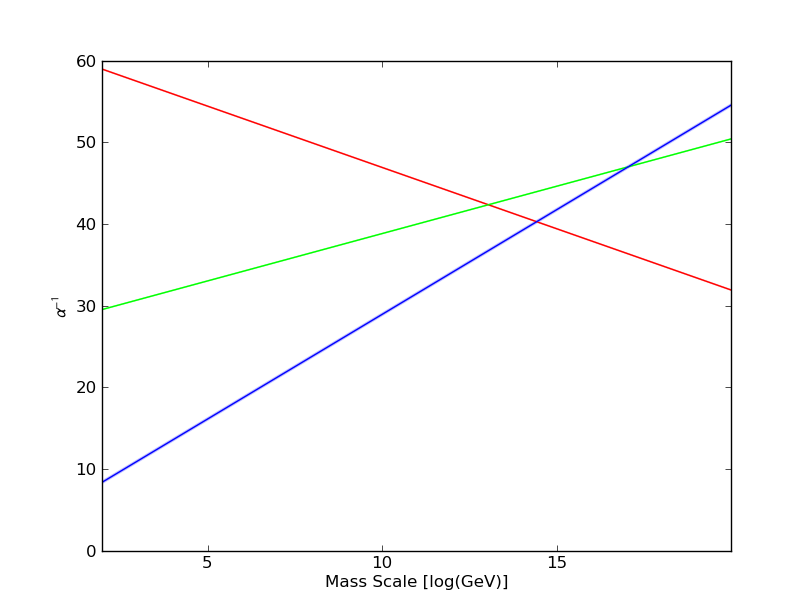
\includegraphics[width=6.75cm]{figs/sm-1.png} & (b) 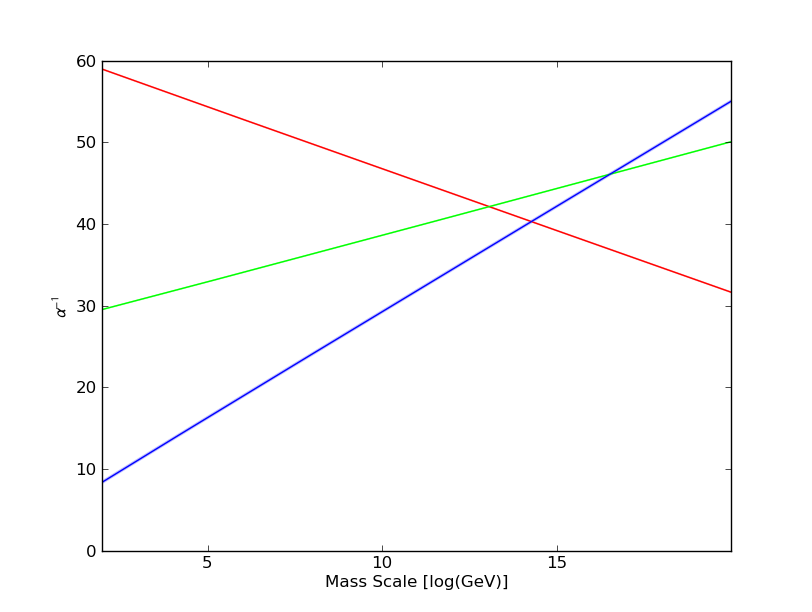
\includegraphics[width=6.75cm]{figs/sm-2.png} \\
(c) 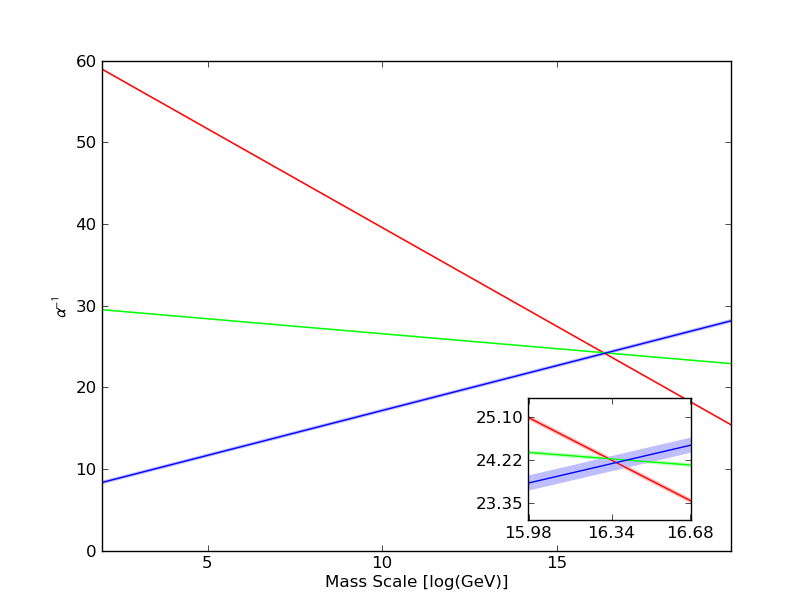
\includegraphics[width=6.75cm]{figs/mssm-1.png} & (d) 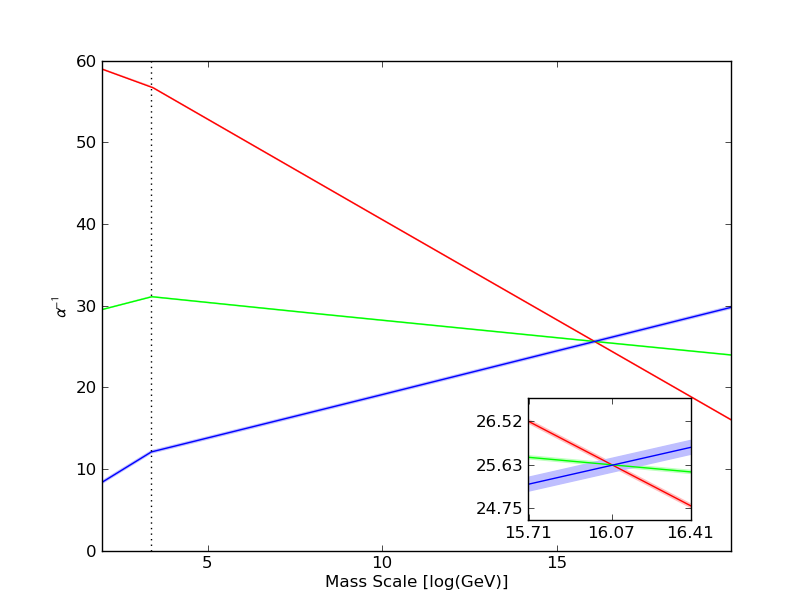
\includegraphics[width=6.75cm]{figs/mssm-2.png} \\
\end{tabular}
\caption[]{Graphs of running coupling obtained from the forward propagation (FP) method, described in the text. (a) SM, 1 loop (b) SM, 2 loops (c) MSSM, 1 loop [$\overrightarrow{\chi}^2_\mathrm{min} = 2.881$ to 3sf] (d) MSSM, 2 loops [$\overrightarrow{\chi}^2_\mathrm{min} = 0.0176$ to 3sf].}
\label{fig:nofit}
\end{center}
\end{figure}

Figure \ref{fig:nofit} shows the results of using the FP method for the SM and MSSM at one and two loops. From the figure, we can deduce that the SM does not admit unification up to two loops. The MSSM is more promising: despite not requiring unification (only minimisation of Eqn. \ref{eqn:susy-min-fp}), for the 2-loop MSSM (Fig. \ref{fig:nofit}d)  $\overrightarrow{\chi}^2_\mathrm{min} = 0.0176$ to 3sf; this is not unexpected, as the problem is underconstrained.

Using the BP method for the two-loop MSSM, the parameters $M_\mathrm{SUSY}$, $M_\mathrm{GUT}$ and $\alpha_\mathrm{GUT}$ were allowed to vary. The parameter space is mapped in Figure \ref{fig:param-space}. The values corresponding to a minimum of Eqn. \ref{eqn:susy-min-bp} were found using a MCLM algorithm to be
\begin{equation}
M_\mathrm{SUSY} = 10^{(3.39 \pm 0.01)} \, \mathrm{GeV}, \quad
M_\mathrm{GUT} = 10^{(16.10 \pm 0.01)} \, \mathrm{GeV}, \quad
\alpha^{-1}_\mathrm{GUT} = 25.60 \pm 0.02,
\label{eqn:min-bp-params}
\end{equation}
where the errors were determined using $\chi^2 + 1$ error analysis (outlined in the Appendix). Due to the underconstrained nature of this problem, $\overleftarrow{\chi}^2_\mathrm{min}$ was able to reach $\sim 10^{-12}$.

\begin{figure}[th]
\begin{center}
\begin{tabular}{cc}
(a) 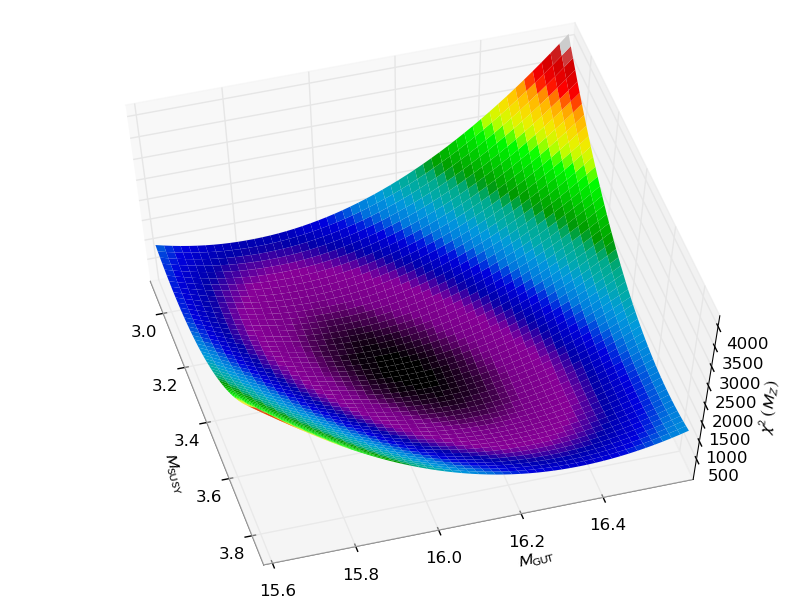
\includegraphics[width=6.75cm]{figs/paramspace-1.png} & (b) 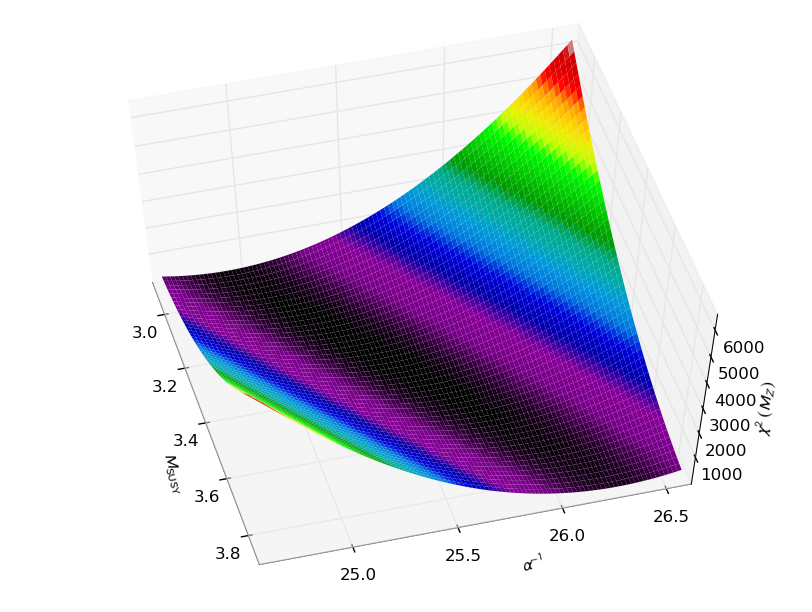
\includegraphics[width=6.75cm]{figs/paramspace-2.png} \\
\multicolumn{2}{c}{(c) 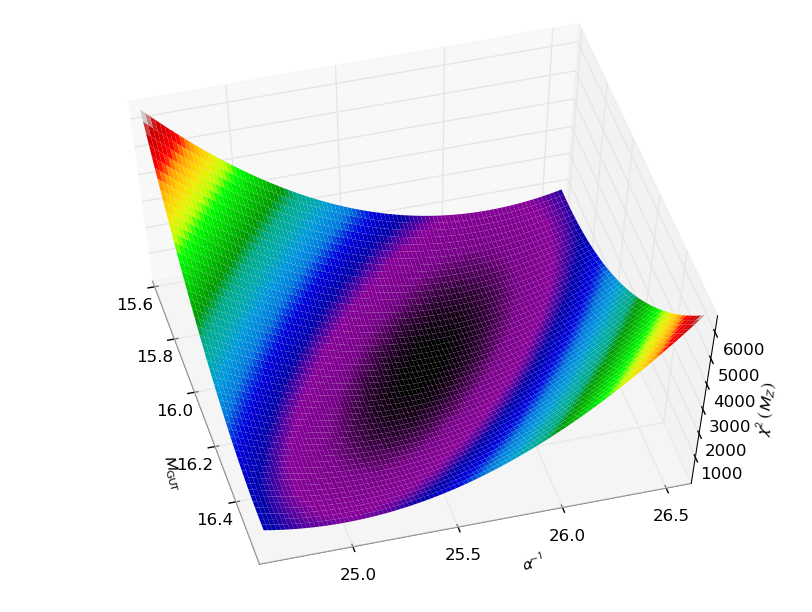
\includegraphics[width=6.75cm]{figs/paramspace-3.png}}
\end{tabular}
\caption[]{3-dimensional plots of the parameter space, related to Eqn. \ref{eqn:susy-min-bp}. In each, one parameter is fixed to the values in Eqn. \ref{eqn:min-bp-params} and the other two are allowed to vary. (a) $\alpha^{-1}_\mathrm{GUT}$ fixed (b) $M_\mathrm{GUT}$ fixed (c) $M_\mathrm{SUSY}$ fixed.}
\label{fig:param-space}
\end{center}
\end{figure}

\section{Discussion}
\subsection{Current Results}
The project appears to be going well - the results found are in accordance with \textit{Amaldi et al.} and are now of better accuracy thanks to the more accurate experimental data from the PDG.

Tests between the Taylor and Integrator methods yielded the same results; however, it is noted that the Integrator method presented more irregularities as we drifted into insoluble areas of the parameter space (see Fig. \ref{fig:psi}). The reasons for this strange behaviour are not obvious, but they can be eliminated by careful choice of the range the parameters are chosen from to do calculation.

\begin{figure}[th]
\begin{center}
\begin{tabular}{cc}
(a) 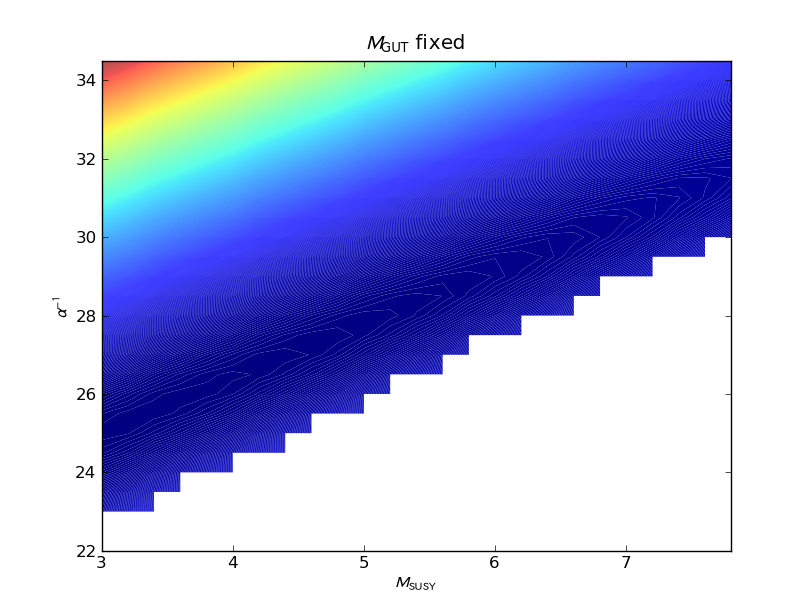
\includegraphics[width=6.75cm]{figs/psi-taylor.png} & (b) 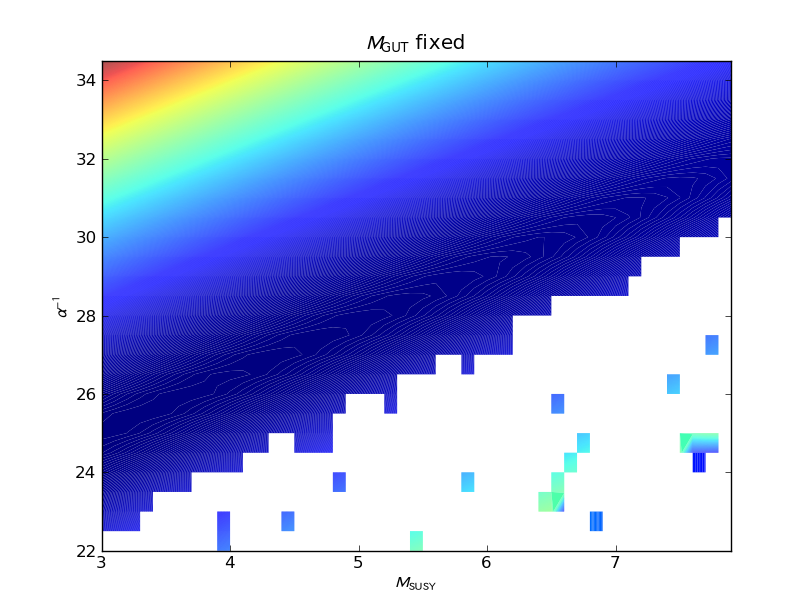
\includegraphics[width=6.75cm]{figs/psi-int.png}
\end{tabular}
\caption[]{Contour plots of the parameter space, with $M_\mathrm{GUT}$ fixed using different methods of solving Eqn. \ref{eqn:rg}, outlined in the text: (a) Using the Taylor method. (b) Using the Integrator method. For both diagrams, the colour represents the value of $\overleftarrow{\chi}^2_\mathrm{min}$, as defined in Eqn. \ref{eqn:susy-min-bp}, with blue areas denote low values and red areas denoting high values. White regions are those where solutions have been rejected, or $\overleftarrow{\chi}^2_\mathrm{min}$ is indeterminable.}
\label{fig:psi}
\end{center}
\end{figure}

\subsection{Future Work}
Now that the ``preliminary'' work has been concluded, the project will now focus on more exotic candidates of GUTs. The changes brought by adding extra dimensions \cite{extra-dims} will be the next step: altering the current implementation to take into account these changes will predict the GUT scale at extra dimensions and analyse whether we will be able to see evidence of extra dimensions at energy scales achievable by the current or next generation of particle accelerators. If this is completed within a reasonable time constraint, further GUTs will be tested.

% Stop double spacing
\singlespace

\begin{thebibliography}{99}
\bibitem{sm-1}{P. S. Wells, \textit{Experimental Tests of the Standard Model}, Eur. Phys. J. C \textbf{33}, S1 (2004), pp. 5-20}
\bibitem{sm-2}{A. Olchevski, M. Winter, \textit{High Precision Tests of the Standard Model and Determination of the Top Quark and Higgs Boson Masses}, C. R. Physique \textbf{3} (2002), pp. 1183-1191}
\bibitem{neutrinos}{M. D. Messier, \textit{Review of Neutrino Oscillation Experiments}, Proceedings of the Flavor Physics and CP Violation Conference, Vancouver (2006)}
\bibitem{mass}{E. Saether, \textit{The Mystery of the Matter Asymmetry}, Beam Line \textbf{26}, SLAC (1996)}
\bibitem{amaldi}{U. Amaldi, W. de Boer, P. H. Frampton, H. F\"{u}rstenau and J. T. Liu, \textit{Consistency Checks of Grand Unified Theories}, Phys. Lett. B \textbf{281} (1992), pp. 374-382}
\bibitem{running-2}{G.M. Prosperia, M. Racitia and C. Simolo, \textit{On the Running Coupling Constant in QCD}, Progress in Particle and Nucl. Phys. \textbf{58}, 2 (2007), pp. 387-438}
\bibitem{pdg}{K. Nakamura et al. (Particle Data Group), \textit{2010 Review of Particle Physics}, J. Phys. G \textbf{37}, 075021 (2010), Section 15: Grand Unified Theories}
\bibitem{bogoliubov}{N. N. Bogoliubov and D. V. Shirkov, \textit{Introduction to the Theory of Quantized Fields}, Wiley (1959), Chapter VIII: The Renormalisation Group}
\bibitem{renorm}{H. Arason, D. J. Castano, B. Keszthelyi, S. Mikaelian, E. J. Piard, P. Ramond, and B. D. Wright, \textit{Renormalization-Group Study of the Standard Model and its Extensions: I. The Standard Model}, Phys. Rev. D \textbf{46} (1992), pp. 3945}
\bibitem{renorm-2}{D. J. Castano, E. J. Piard and P. Ramond, \textit{Renormalization-Group Study of the Standard Model and its Extensions: II. The Minimal Supersymmetric Standard Model}, Phys. Rev. D \textbf{49} (1994), pp. 4882-4901} 
\bibitem{5thirds}{H. Georgi, H. R. Quinn, S. Weinberg, \textit{Hierarchy of Interactions in Unified Gauge Theories}, Phys. Rev. Lett. \textbf{33} (1984), pp. 451-454}
\bibitem{ms}{W. A. Bardeen, A. Buras, D. Duke and T. Muta, \textit{Deep-Inelastic Scattering Beyond the Leading Order in Asymptotically Free Gauge Theories}, Phys. Rev. D \textbf{18} (1978), pp. 3998-4017}
\bibitem{dr}{I. Antoniadis, C. Kounnas, K. Tamvakis, \textit{Simple Treatment of Threshold Effects}, Phys. Lett. B \textbf{119} (1982), pp. 377-380}
\bibitem{b}{M. B. Einhorn and D. R. T. Jones, \textit{The Weak Mixing Angle and Unification Mass in Supersymmetric SU(5)}, Nucl. Phys. B \textbf{196} (1982), pp. 475-488}
\bibitem{odeint}{The SciPy Community, \textit{NumPy and SciPy Documentation}, \url{http://docs.scipy.org/}, retrieved 20th December 2010}
\bibitem{adams}{Press, Teukolsky, Vetterling and Flannery, \textit{Numerical Recipes}, CUP, 3rd Ed. (2007), Chapter 17: Integration of Ordinary Differential Equations}
\bibitem{bdf}{U. M. Ascher and L. R. Petzold, \textit{Computer Methods for Ordinary Differential Equations and Differential-Algebraic Equations}, SIAM (1998), Chapter 10.1.2: BDF and General Multistep Methods}
\bibitem{rosenbrock}{J. R. Palmer, \textit{An Improved Procedure for Orthogonalising the Search Vectors in Rosenbrock's and Swann's Direct Search Optimisation Methods}, The Computer Journal \textbf{12}, 1 (1969), pp. 69-71}
\bibitem{python}{Python Software Foundation, \textit{Python Programming Language}, \url{http://www.python.org}, retrieved 20th December 2010}
\bibitem{scipy}{\texttt{numpy} and \texttt{scipy} are available from \url{http://www.scipy.org/}}
\bibitem{pylab}{J. Hunter, D. Dale, M. Droettboom, \textit{matplotlib - python plotting}, \url{http://matplotlib.sourceforge.net/}}
\bibitem{extra-dims}{K. R. Dienes, E. Dudas and T. Gherghetta, \textit{Grand Unification at Intermediate Mass Scales through Extra Dimensions}, Nuc. Phys. B \textbf{537}, 1-3 (1999), pp. 47-108}
\end{thebibliography}

% Start appendices
\newpage
\appendix

\section{Appendix}

\subsection{Error Propagation}
The couplings in the Standard Model (SM) are given by
\begin{equation}
\alpha_1^{-1} = \dfrac{3}{5} \dfrac{\cos^2 \theta_W}{a} \:, \quad
\alpha_2^{-1} = \dfrac{\sin^2 \theta_W}{a} \:, \quad
\alpha_3^{-1} = \dfrac{1}{a_s}
\label{eqn:coupling}
\end{equation}
and using the world-averaged values
\begin{align}
a^{-1} (M_Z) &= 127.91 \pm 0.02 \nonumber \\
\sin^2 \theta_W (M_Z) &= 0.2312 \pm 0.0002 \\%\label{eqn:couplingexpt} \\
a_s (M_Z) &= 0.119 \pm 0.002 \nonumber
\end{align}
we can determine the running of the couplings. Using $\sigma[x]$ to denote the error in $x$, the errors in each $\alpha_i^{-1}$ are given by
\begin{align}
\sigma[\alpha_1^{-1}] &= \sqrt{\left(\dfrac{3 a^{-1}}{5} \dfrac{\sigma[\sin^2 \theta_W]}{\sqrt{\sin^2 \theta_W}} \right)^2 + \left( \dfrac{\alpha_1^{-1} \sigma[a^{-1}]}{a^{-1}} \right)^2 } \nonumber \\
\sigma[\alpha_2^{-1}] &= \alpha_2^{-1} \sqrt{ \left( \dfrac{\sigma[\sin^2 \theta_W]}{\sin^2 \theta_W} \right)^2 + \left( \dfrac{\sigma[a^{-1}]}{a^{-1}} \right)^2 } \label{eqn:error} \\
\sigma[\alpha_3^{-1}] &= \dfrac{\alpha_3^{-1}}{a_s} \sigma[a_s] \nonumber
\end{align}
where $\sigma[\sin^2 \theta_W]$, $\sigma[a^{-1}]$ and $\sigma[a_s]$ are defined in Eqn.. This implies that
\begin{equation}
\alpha_1^{-1} (M_Z) = 59.00 \pm 0.03 \:, \quad
\alpha_2^{-1} (M_Z) =  29.52 \pm 0.03 \:, \quad
\alpha_3^{-1} (M_Z) =  8.3 \pm 0.1
\label{eqn:couplingvals-a}
\end{equation}

\subsection{$\chi^2 + 1$ Analysis}
In order to determine the error on Eqn. \ref{eqn:min-bp-params}, each parameter in turn was allowed to vary and the other parameters were fixed. The parameter then was then varied until the value of $\chi^2$ reached $\chi^2_\mathrm{min} + 1$, denoting one standard deviation of error; the difference between the parameter value giving $\chi^2_\mathrm{min}$ and this $\chi^2 + 1$ value was taken to be the error.

\subsection{MCLM Algorithm}
The Monte Carlo Levenberg-Marquardt (MCLM) algorithm uses a semi-stochastic method of convergence to find a global minimum of a function. For each trial, random (Monte Carlo) values for the function parameters are chosen; a Levenberg-Marquardt convergence algorithm is then used to converge to the local minimum for that set of initial conditions. This process is then repeated for a number of trials: as the number of trials tends to infinity, the likelihood of obtaining the global minimum approaches certainty.

\end{document}